\chapter{Orbite periodiche}
In questa sezione supponiamo che  $X$ sia uno spazio metrico compatto di dimensione 1 (cio\`e $X=[0,1]$ o $X=S^1$ a meno di omeomorfismo).

\begin{remark}
Le orbite con periodo $p$ corrispondono a punti fissi di $T^p$.
\end{remark}

\section{\texorpdfstring{Partizioni e $T$-grafi}{Partizioni e T-grafi}}
\begin{definition}[Partizione finita]
Sia $\cpa{a_1,\cdots, a_N}$ un insieme finito di punti di $X$ e per ogni $h$ definiamo $J_h=[a_h,a_{h+1}]$.\\ L'insieme $\Jc=\cpa{J_h}$ \`e una \textbf{partizione finita} di $X$ in intervalli se $X=\bigcup_{h=0}^{N-1}J_h$ e 
\[J_h\cap J_k=\begin{cases}
J_h & \text{se }k=h\\
a_{h} & \text{se }k=h-1\\
a_{k} & \text{se }k=h+1\\
\emptyset &\text{altrimenti}
\end{cases}.\] 
\end{definition}

\begin{definition}[Coprire un intervallo $m$ volte]
Sia $m$ un intero positivo e $T:X\to X$ continua. Un intervallo $J_h$ \textbf{ricopre} un intervallo $J_k$ \textbf{(almeno) $m$ volte} se esistono $K_1,\cdots, K_m$ intervalli aperti disgiunti in $J_h$ tali che $T(\ol{K_i})=J_k$ per ogni $i\in\cpa{1,\cdots, m}$.\\
In particolare $J_h$ \textbf{ricopre} $J_k$ se esiste $K\subseteq J_h$ itervallo aperto tale che $T(\ol K)=J_k$.
\end{definition}

\begin{definition}[$T$-grafo associato a partizione]
Data una partizione $\Jc=\cpa{J_1,\cdots, J_N}$ finita in intervalli chiusi, definiamo il \textbf{$T$-grafo associato a $\Jc$} come il grafo orientato che ha come vertici gli indici $\cpa{1,\cdots, N}$ e colleghiamo due vertici con una freccia orientata $m:h\to k$ se $J_h$ ricopre $J_k$ almeno una volta.
\end{definition}
\begin{remark}
\`E possibile definire una variante graduata del $T$-grafo dove il grado di $h\to k$ registra quante volte $J_h$ ricopre $J_k$.
\end{remark}

\begin{definition}[Cammino ammissibile su $T$-grafo]
Un \textbf{cammino ammissibile} sul $T$-grafo associato ad una partizione $\Jc$ \`e una successione di intervalli di $\Jc$ tale che la sequenza di indici ha la propriet\`a che due indici successivi $hk$ possono presentarsi solo se esiste una freccia orientata $h\to k$ nel $T$-grafo associato (cio\`e solo se $J_h$ ricopre $J_k$ almeno una volta).
\end{definition}

\begin{example}[Un $T$-grafo]
Consideriamo una funzione $T:[0,1]\to[0,1]$ data da 
\begin{figure}[!htb]
	\centering
	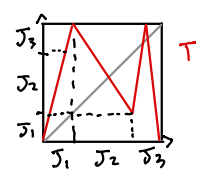
\includegraphics[width=4cm]{Immagini/esempio_Grafico_per_TGrafo.png}
	\caption{Esempio di una funzione. Notiamo che $J_1$ ricopre $J_1,\ J_2$ e $J_3$, $J_2$ ricopre $J_2$ e $J_3$ e $J_3$ ricopre $J_1,\ J_2$ e $J_3$.}
\end{figure}
Il $T$-grafo associato \`e\footnote{i numeri sulle frecce indicano quante volte un intervallo ricopre un altro}
\[\begin{tikzcd}
	1 \arrow[loop left] && 2\arrow[loop right] \\
	& 3\arrow["{_2}", loop below]
	\arrow[curve={height=6pt}, from=2-2, to=1-1]
	\arrow[curve={height=6pt}, from=1-1, to=2-2]
	\arrow["{_2}", curve={height=-6pt}, from=2-2, to=1-3]
	\arrow[curve={height=-6pt}, from=1-3, to=2-2]
	\arrow[curve={height=-6pt}, from=1-1, to=1-3]
\end{tikzcd}\]
Un esempio di cammino ammissibile \`e $J_1J_2J_3J_3J_1J_1$, mentre $J_1J_2J_1$ non \`e ammissibile perch\'e $J_2$ non ricopre $J_1$.
\end{example}

\begin{proposition}[Criterio con grafo per esistenza di orbite periodiche]\label{CriterioTGrafoPerEsistenzaOrbitePeriodiche}
Sia $T:X\to X$ continua, $X$ compatto di dimensione $1$ e $\Jc=\cpa{J_1,\cdots, J_N}$ partizione finita di $X$. Considerando il $T$-grafo associato a $\Jc$, se esiste un cammino ammissibile 
\[J_{p(1)}J_{p(2)}\cdots J_{p(s+1)}\] 
di lunghezza $s+1$ chiuso (cio\`e $p(1)=p(s+1)$) allora esiste $x\in J_{p(1)}$ tale che $T^s(x)=x$ e $T^i(x)\in J_{p(i+1)}$ per ogni $i$.
\end{proposition}
\begin{proof}
Poniamo $\ol K_{s+1}=J_{p(s+1)}$. Poich\'e il cammino \`e ammissibile, $J_{p(s)}$ copre $J_{p(s+1)}$ almeno una volta, quindi esiste $K_s\subseteq J_{p(s)}$ tale che $T(\ol K_s)=J_{p(s+1)}=\ol K_{s+1}$.\\
Similmente esiste $\wt K_{s-1}\subseteq J_{p(s-1)}$ tale che $T(\ol{\wt K_{s-1}})=J_{p(s)}$, quindi restringendo opportunamente troviamo un intervallo $K_{s-1}\subseteq J_{p(s-1)}$ tale che 
\[T(\ol K_{s-1})=\ol K_s\subseteq J_{p(s)}.\]
Reiterando costruiamo $K_1,\cdots, K_s$ aperti in $X$ tali che $K_i\subseteq J_{p(i)}$ e $T(\ol K_i)=\ol K_{i+1}$ (in particolare $T^{s-i+1}(\ol K_i)=\ol K_{s+1}$). Questo mostra che $T^s(\ol K_1)=\ol{K_{s+1}}=J_{p(s+1)}=J_{p(1)}$, quindi per il il teorema del valore intermedio $T^s\res{\ol K_1}$ ha un punto fisso, cio\`e esiste $x\in \ol K_1\subseteq J_{p(1)}$ tale che $T^s(x)=x$.\\
Per concludere basta osservare che per costruzione $T^i(x)\in \ol K_{i+1}\subseteq J_{p(i+1)}$.
\end{proof}
\begin{remark}
\`E possibile che il punto fisso di periodo $s$ trovato abbia periodo minimo che divide strettamente $s$.
\end{remark}
\begin{remark}[Criterio di esistenza per periodi minimi]\label{CriterioEsistenzaPeriodiMinimi}
Se il cammino NON \`e della forma
\[\under{s/k\text{ volte}}{(J_{p(1)}J_{p(2)}\cdots J_{p(k)}) \cdots (J_{p(1)}J_{p(2)}\cdots J_{p(k)})}J_{p(1)}\]
allora il punto $x$ trovato nel teorema ha periodo \textit{minimo} $s$.\\
In particolare se il cammino attraversa sempre indici diversi prima di tornare a $J_{p(1)}$ allora $x$ ha periodo minimo $s$. 
\end{remark}
\begin{remark}
Se $T$ \`e continua eccetto in un numero finito di punti possiamo provare a infittire la partizione e stando attenti al comportamento sul bordo la proposizione (\ref{CriterioTGrafoPerEsistenzaOrbitePeriodiche}) continua in genere a valere.
\end{remark}

\section{Teorema di Sharkovsky}
\subsection{Ordinamento e teorema}
\begin{definition}[Ordinamento di Sharokovsky]
Definiamo l'\textbf{ordinamento di Sharokovsky} su $\N^+$ (che indichiamo $(\N^+,\prec)$) come segue:\\ 
Siano $a,b$ dispari e $p,q\in\N$. Poniamo
\[2^pa\prec 2^qb\coimplies \begin{cases}
a\neq 1\neq b,\ p>q\text{ oppure}\\
a\neq 1\neq b,\ p=q,\ a>b\text{ oppure}\\
a=1,\ b\neq 1\text{ oppure}\\
a=b=1,\ p<q.
\end{cases}\]
Pi\`u graficamente:
\begin{align*}
1\prec2^2\prec 2^3\prec\cdots&\\
\vdots&\\
\cdots\prec2^2\cdot7\prec2^2\cdot5\prec2^2\cdot3&\\
\cdots\prec2\cdot7\prec2\cdot5\prec2\cdot3&\\
\cdots\prec7\prec5\prec3&
\end{align*}
\end{definition}
\begin{remark}
L'ordine di Sharkovsky \`e un ordine totale su $\N^+$.
\end{remark}

\begin{theorem}[Sharkovsky]\label{TeoremaSharkovsky}
Se $T:[a,b]\to [a,b]$ \`e continua ed esiste un'orbita periodica di periodo minimo $m$ allora esiste un'orbita periodica di periodo minimo $n$ per ogni $n\prec m$.
\end{theorem}
\begin{proof}[Dimostrazione (in programma solo il caso $m$ dispari).]
Se $m=1$ la tesi \`e evidente. Consideriamo il caso di $m$ dispari maggiore di $1$. In tal caso $n\prec m$ equivale a dire $n=1$, $n>m$ oppure $n<m$ e $n$ pari.\\
Supponiamo senza perdita di generalit\`a che non esista orbita periodica di periodo minimo $\wt m$ per ogni $\wt m$ tale che $\wt m\succ m$, infatti, poich\'e $m$ \`e dispari, esistono solo un numero finito di $\wt m$ tali che $\wt m\succ m$, basta considerare il massimo (rispetto a $\prec$, quindi il minimo per $<$).\\
Sia $P_1$ un punto periodico con periodo minimo $m$ e sia
\[\Oc(P_1)=\cpa{P_1,P_2,\cdots, P_m},\]
dove ordiniamo $a \leq P_1 < P_2 < \cdots < P_m \leq b$. Poniamo
\[\Jc=\cpa{J_h}_{h\in\cpa{1,\cdots, m-1}}\cup \cpa{[a,P_1], [P_m,b]},\]
dove $J_h=[P_h,P_{h+1}]$. Seguiamo alcuni passi:
\setlength{\leftmargini}{0cm}
\begin{enumerate}
\item Notiamo che necessariamente $T(P_1)>P_1$ e $T(P_m)<P_m$. Sia allora $\ol h$ l'indice tale che $T(P_r)<P_r$ per ogni $r>\ol h$ e $T(P_{\ol h})>P_{\ol h}$ \footnote{esiste per il principio del minimo}. 

\begin{figure}[!htb]
	\centering
	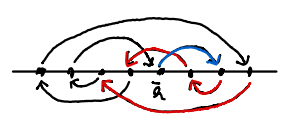
\includegraphics[width=7cm]{Immagini/Definizione_hbarra.png}
	\caption{Rappresentazione grafica della definizione di $\ol h$.}
\end{figure}

Osserviamo che $T(P_{\ol h})\geq P_{\ol h+1}$ e $T(P_{\ol h+1})\leq P_{\ol h-1}$, quindi $J_{\ol h}$ ricopre se stesso. Segue dunque che $J_{\ol h}J_{\ol h}$ \`e un cammino ammissibile e quindi per la proposizione (\ref{CriterioTGrafoPerEsistenzaOrbitePeriodiche}) esiste un punto fisso in $J_{\ol h}$, quindi abbiamo verificato l'esistenza di un'orbita di \textit{periodo minimo 1}.

\item \underline{Claim:} se $J_h$ ricopre se stesso allora per ogni $\ell\in \cpa{1,\cdots, m-1}$ esiste un cammino ammissibile da $J_{h}$ a $J_{\ell}$:

Poniamo $V_1=\cpa{h}$ e per ogni $k\geq1$ poniamo 
\[V_{k+1}=\cpa{v\in \cpa{1,\cdots, m-1}\mid \exists w\in V_k\ t.c.\ J_w\text{ ricopre }J_v}.\]
Poich\'e $J_{h}$ ricopre se stesso si ha che $V_k\subseteq V_{k+1}$ per ogni $k\geq 1$, quindi esiste $\ol k$ tale che $V_{\ol k}=V_{\ol k+1}=V_r$ per ogni $r\geq \ol k+1$. Si presentano due possibilit\`a:
\begin{itemize}
\item $V_{\ol k}=\cpa{1,\cdots,m-1}$ e abbiamo completato il passo,
\item $V_{\ol k}$ \`e un sottoinsieme stretto di $\cpa{1,\cdots, m-1}$.
\end{itemize} 
Mostriamo che la seconda non pu\`o verificarsi:\\
Per assurdo supponiamo $V_{\ol k}\subsetneq \cpa{1,\cdots, m-1}$, allora partendo da $h$ esiste un intervallo che non viene ricoperto (per esempio $J_a$). Notiamo che $\bigcup_{I\in V_k}I= T^k(J_{h})$ \`e un intervallo, infatti l'immagine tramite una mappa continua di uno spazio connesso \`e connessa. Poich\'e $J_{h}\subseteq T^k(J_{h})$ per ogni $k$ si ha che se $J_{a}$ non viene ricoperto allora $P_a$ o $P_{a+1}$ non pu\`o mai essere immagine di $P_{h}$, ma questo \`e assurdo perch\'e $P_a,P_{a+1}\in \Oc(P_1)=\Oc(P_{h})$.
\item \underline{Claim:} Esiste $J_{\ol \ell}$ con $\ol \ell\neq \ol h$ che ricopre $J_{\ol h}$.

Per assurdo supponiamo che non esista un tale $\ol\ell$. Sotto questa ipotesi mostriamo che $T(\cpa{P_{\ol{h}+1},\cdots,P_m})\subseteq \cpa{P_1,\cdots, P_{\ol h}}$ e $T(\cpa{P_1,\cdots, P_{\ol h}})\subseteq \cpa{P_{\ol{h}+1},\cdots,P_m}$:\\
Poich\'e $T(P_{\ol h+1})\leq P_{\ol h}$ necessariamente questo \`e il caso anche per $T(P_{\ol h+2})$, altrimenti $J_{\ol h+1}$ ricoprirebbe $J_{\ol h}$. Procedendo per induzione andando verso $P_m$ abbiamo mostrato la prima inclusione. L'altra segue in modo analogo notando che $T(P_{\ol h})\geq P_{\ol h+1}$ e procedendo per induzione verso $P_1$.

Abbiamo quindi diviso i punti esattamente a met\`a, ma questo \`e assurdo perch\'e $m$ dispari.
\item Unendo i due punti precedenti esiste un cammino ammissibile della forma
\[J_{\ol h}J_{p(2)}\cdots J_{p(s)}J_{\ol h}\]
tale che $p(i)\neq \ol h$ per qualche $i\in\cpa{2,\cdots, s}$.\\
Mostriamo che un cammino ammissibile di lunghezza minima di questa forma \`e tale che $s=m-1$:
\setlength{\leftmargini}{0cm}
\begin{itemize}
\item[$\boxed{s\geq m-1}$] Per assurdo supponiamo $s<m-1$. Se $s$ \`e dispari allora per la proposizione (\ref{CriterioTGrafoPerEsistenzaOrbitePeriodiche}) esiste $x\in J_{\ol h}$ tale che $T^s(x)=x$, ma questo \`e assurdo perch\'e, poich\'e $s<m$ \`e dispari, $s\leq m-2$ e quindi $T$ ammetterebbe un'orbita con periodo minimo dispari\footnote{potenzialmente un divisore di $s$} minore di $m$.\\
Se $s$ \`e pari allora il cammino 
\[J_{\ol h}J_{p(2)}\cdots J_{p(s)}J_{\ol h}J_{\ol h}\]
\`e ammissibile e quindi troviamo $x\in J_{\ol h}$ tale che $T^{s+1}(x)=x$, ma questo \`e assurdo perch\'e $s<m-1$ e $m-1$ pari implica che $s\leq m-3$ e quindi $s+1\leq m-2$ e abbiamo lo stesso assurdo di prima.
\item[$\boxed{s=m-1}$] Visto il punto precedente basta mostrare che il cammino contiene ogni $J_{\ell}$ per $\ell\in\cpa{1,\cdots, m-1}$ al massimo una volta (escluso l'ultimo $J_{\ol h}$). Se $J_\ell$ apparisse pi\`u volte potremmo eliminare il tratto tra la prima e l'ultima manifestazione di $J_\ell$\footnote{per esempio per $\ell=1$ e $\ol h=1$ si avrebbe $J_1J_2J_3J_4J_2J_3J_3J_1\leadsto J_1J_2J_3J_3J_1$} e trovare un cammino ammissibile pi\`u breve, negando la minimalit\`a del cammino di partenza.
\end{itemize}
\setlength{\leftmargini}{0.5cm}

\item \underline{Claim:} Esiste un unico $\ell\in\cpa{1,\cdots,m-1}\bs\cpa{\ol h}$ tale che $J_\ell$ ricopre $J_{\ol h}$.\\
Abbiamo gi\`a mostrato l'esistenza quindi supponiamo per assurdo che esistano $k_1\neq k_2$ diversi da $\ol h$ tali che $J_{k_1}$ e $J_{k_2}$ ricoprono $J_{\ol h}$. In tal caso, preso un cammino ammissibile come nel punto precedente si avrebbe che se due indici distinti coprono $J_{\ol h}$ allora esisterebbe un cammino ammissibile pi\`u breve, contraddicendo il punto precedente.

\item Combinando i due punti precedenti ricaviamo che se $V_1=\cpa{\ol h}$ e costruiamo gli insiemi di indici come al punto 2, ad ogni applicazione successiva di $T$ viene aggiunto esattamente un indice fino a raggiungere $\cpa{1,\cdots, m-1}$.\\
Imponiamo allora come notazione $I_1=J_{\ol h}$, $I_2=J_{p(2)}$ dove $\cpa{p(2)}=V_2\bs V_1$ e procedendo iterativamente. In questa notazione si ha che il cammino\footnote{siamo giustificati nel chiamarlo ``il cammino" per l'osservazione appena fatta.} pi\`u breve ammissibile che parte da $J_{\ol h}$ e torna a $J_{\ol h}$ passando per un altro intervallo \`e dato da
\[I_1I_2\cdots I_{m-1}I_1.\]

\item Osserviamo che, affinch\'e $I_1\cdots I_{m-1}I_1$ abbia la propriet\`a di lunghezza minima mostrata, $I_1$ copre solo $I_1$ e $I_2$. Similmente $I_2$ pu\`o coprire al massimo $I_1,\ I_2$ e $I_3$ eccetera. Osserviamo dunque che $I_2=J_{\ol h+1}$ oppure $J_{\ol h-1}$, senza perdita di generalit\`a supponiamo $I_2=J_{\ol h-1}$\footnote{il ragionamento procede in modo simile per l'altro caso}. Si deve dunque avere che $T(P_{\ol h+1})=P_{\ol h-1}$ e $T(P_{\ol h})=P_{\ol h+1}$. Imponendo iterativamente le condizioni sopra ricaviamo che $I_2$ copre solo $I_3$, $I_3$ copre solo $I_4$ e cos\`i procedendo fino a raggiungere $I_{m-1}=J_{1}$, la cui immagine forzata ad essere $[P_{\ol h},P_m]$ cio\`e, sempre per la corrispondenza esplicita trovata, $I_1\cup I_2\cup \cdots\cup I_{m-2}$.
\begin{figure}[!htb]
	\centering
	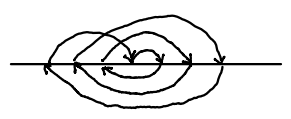
\includegraphics[width=7cm]{Immagini/Disegno_A.png}
	\caption{Rappresentazione di come i punti dell'orbita sono organizzati. Il punto centrale \`e $\ol h$. La figura rappresenta il caso di $I_2=J_{\ol h-1}$, l'altro caso \`e dato riflettendo l'immagine attraverso un asse verticale.}
	\label{ConfigurazioneOrbita}
\end{figure}

\item Mostriamo che esiste un'orbita periodica di \textit{periodo minimo $n$ per ogni $n>m$}:\\
Notiamo che il cammino
\[\under{m-1}{I_1\cdots I_{m-1}}\under{n-m+2}{I_1\cdots I_1}\]
\`e ammissibile per il punto precedente e quindi per (\ref{CriterioEsistenzaPeriodiMinimi}) esiste $x$ tale che $T^{n}(x)=x$ dove $n$ \`e il periodo minimo.

\item Mostriamo che esiste un'orbita periodica di \textit{periodo minimo $n$ per ogni $n<m$ pari}.\\
\`E sufficiente mostrare che $I_{m-1}$ ricopre $I_k$ per ogni $k$ dispari, infatti in tal caso baster\`a applicare (\ref{CriterioEsistenzaPeriodiMinimi}) ai cammini ammissibili della forma
\[I_{m-1}I_k I_{k+1}\cdots I_{m-2}I_{m-1}\]
per ogni $k$ dispari.
\end{enumerate}
Consideriamo ora il caso $m$ pari\footnote{\textbf{Da qu\`i in poi \`e una curiosit\`a che non fa parte del programma.}}.
Senza perdita di generalit\`a supponiamo che $T$ abbia un'orbita di periodo minimo $m$ e non di periodo $k$ per ogni $k\succ m$. Scriviamo $m=2^p\wt m$.\\
Seguendo quanto fatto per il caso dispari mostriamo anche in questo caso che $J_{\ol h}$ ricopre se stesso e che iterando $T$ ricopre ogni intervallo. Applicando il caso dispari a $T^{2^p}$ e $\wt m$ troviamo per ogni $k\prec \wt m$ un valore $x$ tale che $x$ abbia periodo minimo $k$ per $T^{2^p}$, e quindi ha periodo $2^pk$ per $T$. Per mostrare che questo periodo \`e minimo \`e necessario studiare pi\`u approfonditamente l'equivalente dei punti 3, 4 e 5.
\end{proof}

Il teorema di Sharkovsky segna una netta distinzione qualitativa tra mappe su intervalli e mappe su circonferenze:

\begin{proposition}[Punti periodici su $S^1$]
Sia $T:S^1\to S^1$ un omeomorfismo, allora se esiste un punto di periodo minimo $p$ ogni punto periodico \`e di periodo minimo $p$.
\end{proposition}
\begin{proof}
NON DATA DURANTE IL CORSO
\end{proof}